\section{Honig's analysis model of data structures}
\label{appendixA}

In his dissertation \textcite{Honig1975} developed an analysis model of data
structures based on a review of 21 programming languages and data base
management systems.  A partial summary of the model is given by
\textcite{Honig1978}.  In Honig's analysis model ``data structures are divided
into three classes (aggregates, associations, and files) and each class is
modeled with a set of questions. Each question delinates one significant
characteristic of the data structure and can be viewed as one axis of a
n-dimensional universe of data structures.'' This appendix includes a copy of
these questions for better comparision, as applied in
section~\ref{sec:honig}.

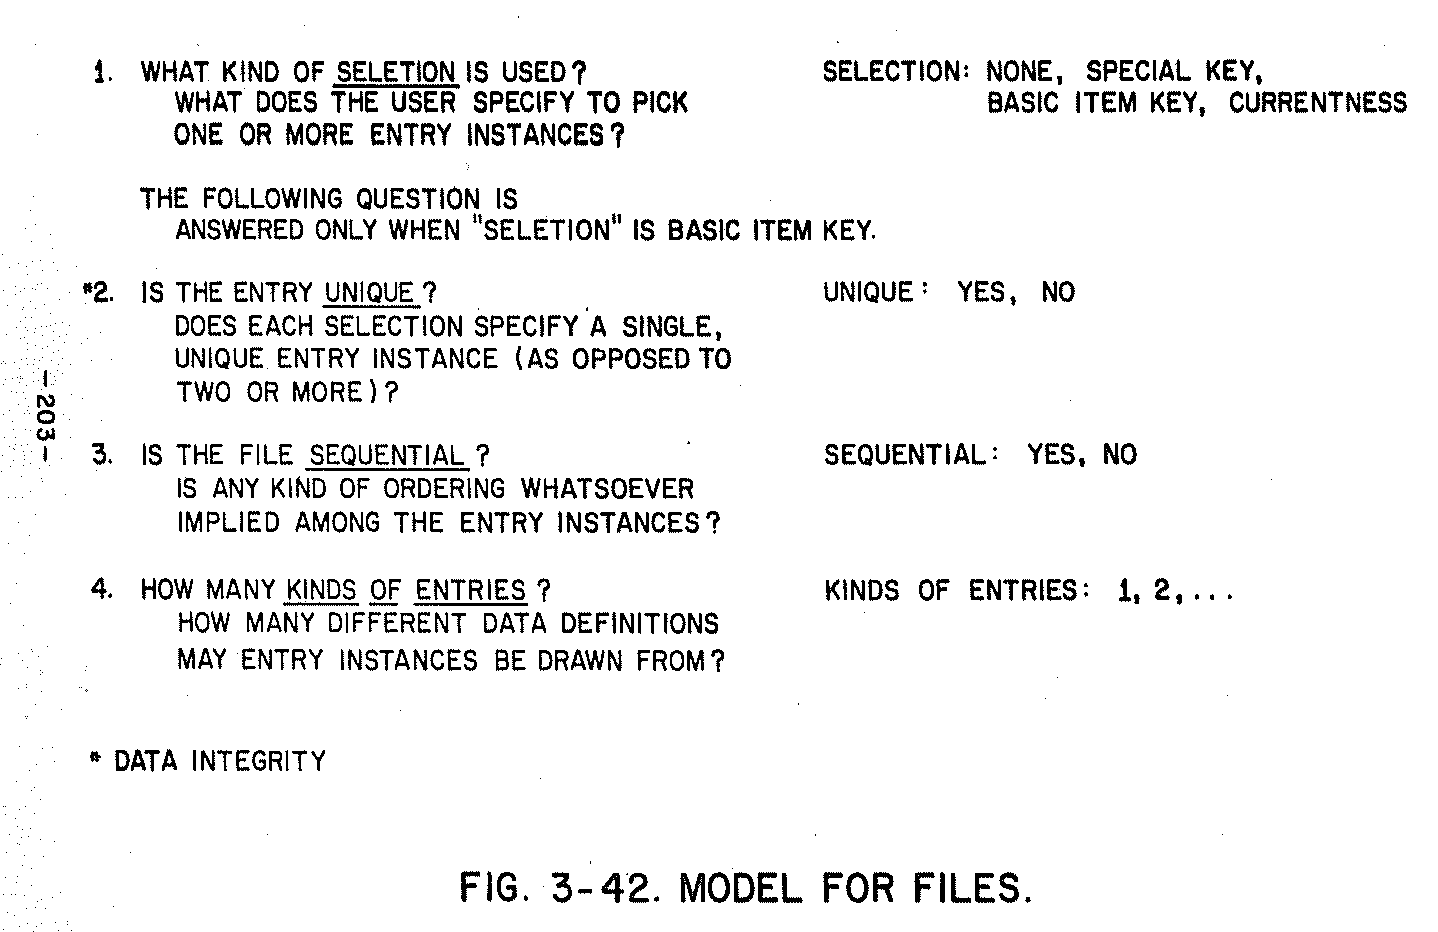
\includegraphics[width=\textwidth]{img/honig1975fig3-42.png}

\thispagestyle{empty}
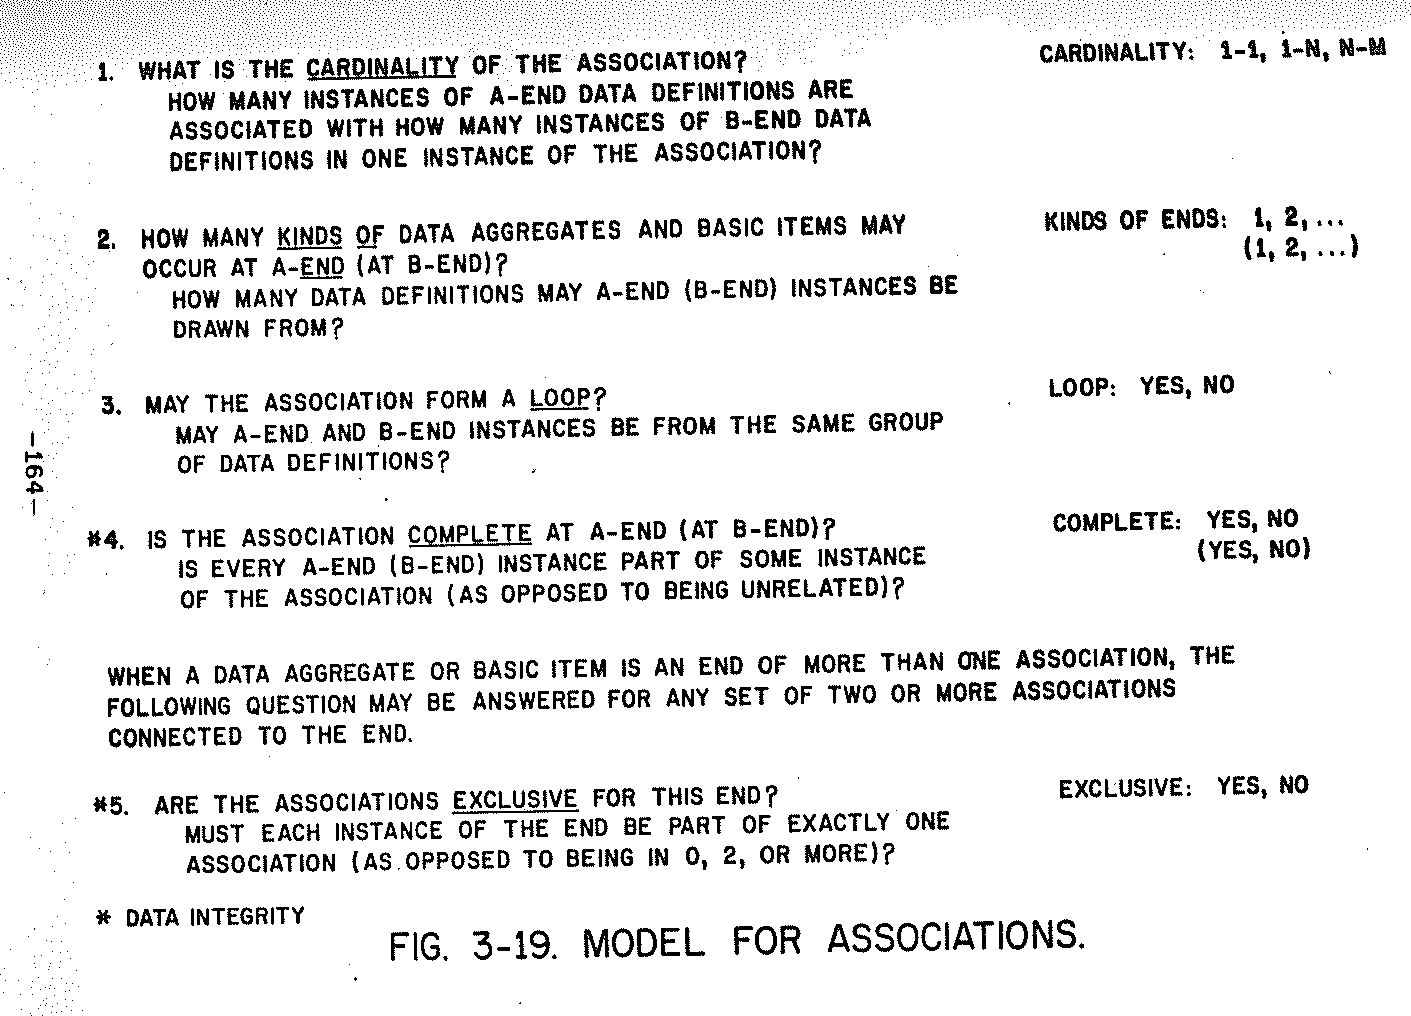
\includegraphics[width=0.9\textwidth]{img/honig1975fig3-19.png}

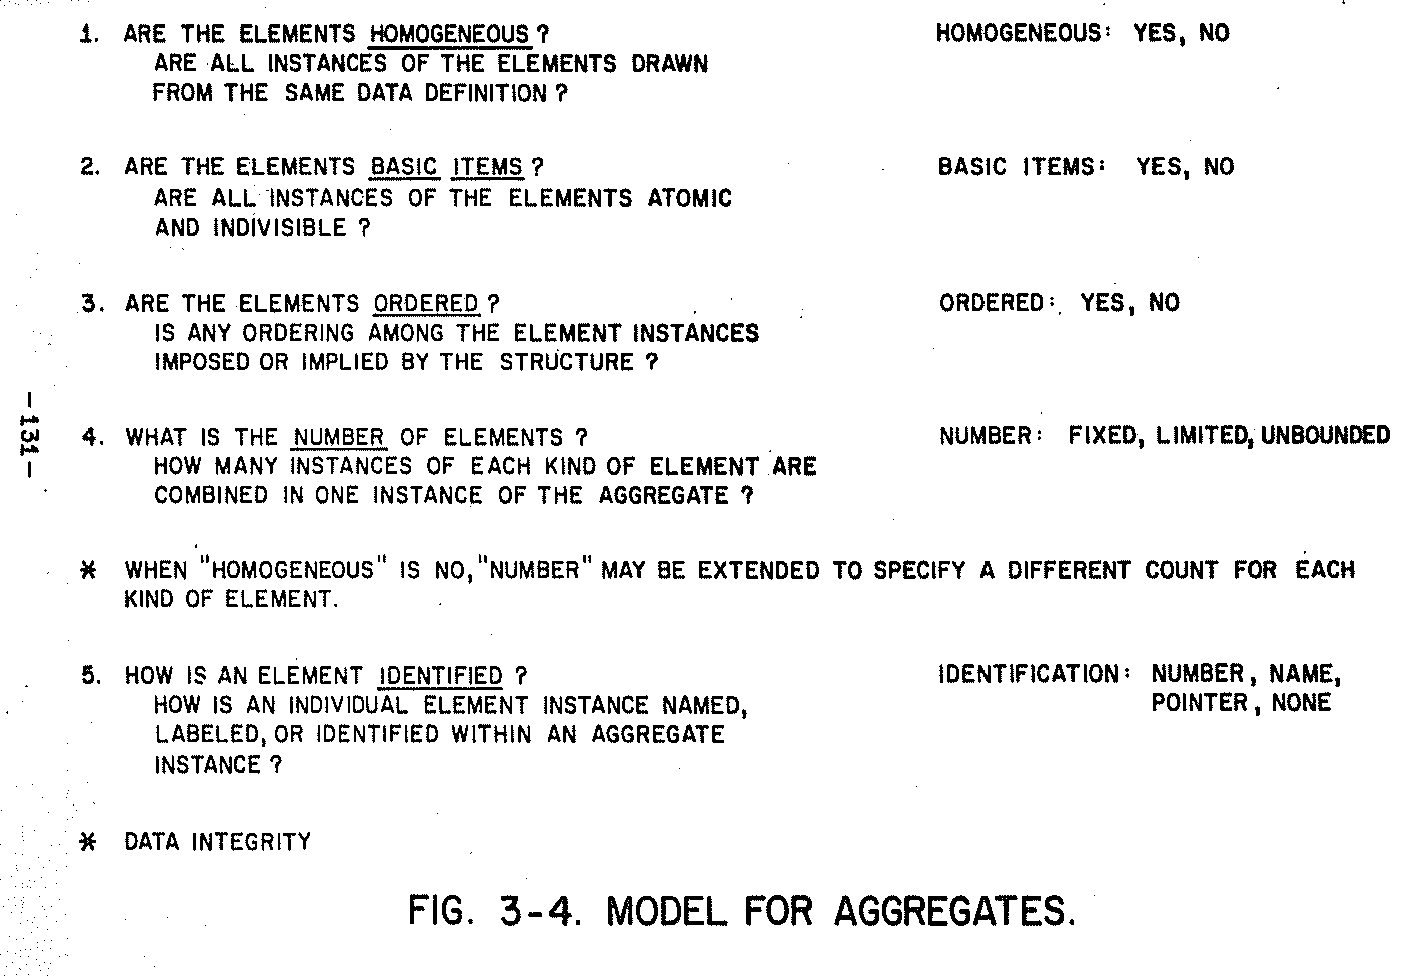
\includegraphics[width=0.9\textwidth]{img/honig1975fig3-4.png}
